\documentclass[conference]{IEEEtran}
\IEEEoverridecommandlockouts

% Packages
\usepackage{cite}
\usepackage{amsmath,amssymb,amsfonts}
\usepackage{algorithmic}
\usepackage{graphicx}
\usepackage{textcomp}
\usepackage{xcolor}
\usepackage{booktabs}
\usepackage{multirow}
\usepackage{tikz}
\usetikzlibrary{shapes.geometric, arrows.meta, positioning, fit, backgrounds}
\usepackage{url}

\def\BibTeX{{\rm B\kern-.05em{\sc i\kern-.025em b}\kern-.08em
    T\kern-.1667em\lower.7ex\hbox{E}\kern-.125emX}}

\begin{document}

\title{PAIR: Perceptual Adaptive Importance-Guided ROI Compression\\An Exploratory Investigation}

\author{\IEEEauthorblockN{Abir Gupta}
\IEEEauthorblockA{\textit{Independent Researcher}\\
Bengaluru, India \\
abir.guptaaa@gmail.com}}

\maketitle

\begin{abstract}
This paper presents PAIR (Perceptual Adaptive Importance-guided ROI), a novel image compression framework that combines multi-component perceptual importance mapping with JPEG 2000's Region of Interest (ROI) coding. Unlike existing approaches that rely on single-component saliency or manual ROI specification, PAIR automatically generates importance-driven quality allocation through integration of edge detection, texture analysis, and visual saliency. We conduct comprehensive evaluation on the Kodak dataset, comparing PAIR against established codecs (JPEG, WebP) and analyzing the challenges of translating perceptual models into compression gains. While PAIR achieves +1.77 dB improvement over naive perceptual approaches, it remains 1.65 dB below JPEG at Q70, with the gap widening to 3.92 dB at Q95. Our subsequent implementation with tile-based ROI encoding via OpenJPEG reverses this trend at higher quality levels, achieving PSNR of 43.70 dB at Q95 (2.91 dB above JPEG). Our analysis provides valuable insights into the gap between perceptual modeling and practical rate-distortion optimization, and demonstrates that proper ROI implementation can yield measurable gains.
\end{abstract}

\begin{IEEEkeywords}
Image compression, JPEG 2000, ROI coding, perceptual importance, visual saliency, empirical analysis
\end{IEEEkeywords}

\section{Introduction}

The human visual system exhibits highly non-uniform sensitivity to image content, with greater attention to edges, textured regions, and salient objects~\cite{wang2004image}. This observation has motivated decades of research into perceptual image compression: can we allocate bits according to human visual importance rather than uniform quantization?

Existing perceptual compression methods typically fall into two categories: (1) single-component saliency-based approaches~\cite{guo2010visual} that identify important regions through bottom-up attention models, or (2) deep learning methods~\cite{balle2018variational} that learn compression mappings end-to-end. The former often lack comprehensive perceptual modeling, while the latter require extensive training data and lack interpretability.

This paper investigates a third path: \textbf{can multi-component perceptual importance mapping, integrated with proven compression technology, yield competitive performance?} We propose PAIR (Perceptual Adaptive Importance-guided ROI), which combines:

\begin{enumerate}
    \item \textbf{Multi-Component Importance Framework}: Fusion of edge strength, texture complexity, and visual saliency into unified importance maps
    \item \textbf{Automatic ROI Generation}: Adaptive tier-based quality allocation without manual specification
    \item \textbf{JPEG 2000 Integration}: Leveraging optimized entropy coding while adding perceptual guidance
\end{enumerate}

Through rigorous benchmarking on the Kodak dataset~\cite{kodak}, we find that \textit{explicit perceptual importance mapping faces fundamental challenges}. While PAIR improves upon naive approaches, it underperforms standard codecs, revealing insights about the limitations of perceptual compression.

\textbf{Contributions:}
\begin{itemize}
    \item First comprehensive multi-component importance framework for JPEG 2000 ROI coding
    \item Rigorous empirical evaluation on standard benchmarks
    \item Analysis of why perceptual approaches struggle to compete with established codecs
    \item Insights for future perceptual compression research
\end{itemize}

\section{Related Work}

\subsection{Perceptual Image Coding}

Visual saliency-based compression~\cite{guo2010visual} allocates higher bitrates to salient regions identified through spectral residual or graph-based models. Just-Noticeable-Difference (JND) approaches~\cite{wu2017just} estimate perceptual thresholds for quantization noise. These methods demonstrate perceptual quality improvements but often at the cost of objective metrics.

Recent deep learning approaches~\cite{balle2018variational,minnen2018joint} achieve state-of-the-art compression through learned transforms and entropy models, but require substantial computational resources and training data. Our work explores whether classical computer vision techniques can provide competitive perceptual guidance.

\subsection{JPEG 2000 and ROI Coding}

JPEG 2000~\cite{taubman2002jpeg2000} uses wavelet transforms with sophisticated embedded block coding (EBCOT), achieving superior rate-distortion over DCT-based JPEG. The standard supports Region of Interest (ROI) coding through the Maxshift method, allowing specified regions to receive higher quality.

However, standard JPEG 2000 relies on uniform quality allocation or manual ROI specification. Our contribution is \textit{automatic ROI generation} from multi-component perceptual analysis, eliminating manual annotation while attempting to improve perceptual quality.

\subsection{Multi-Component Perceptual Models}

While individual perceptual features (edges, saliency, texture) are well-studied, their integration for compression guidance remains underexplored. Wang et al.~\cite{wang2004image} demonstrated that structural similarity (SSIM) correlates better with perception than MSE, suggesting multi-component analysis is valuable. Our work empirically tests whether this translates to compression gains.

\section{Methodology}

\subsection{Algorithm Overview}

PAIR operates in four stages: (1) perceptual importance map generation, (2) ROI tier segmentation, (3) quality allocation, and (4) JPEG 2000 encoding with importance-guided parameters. Figure~\ref{fig:flowchart} illustrates the complete workflow.

\begin{figure*}[t]
\centering
\small
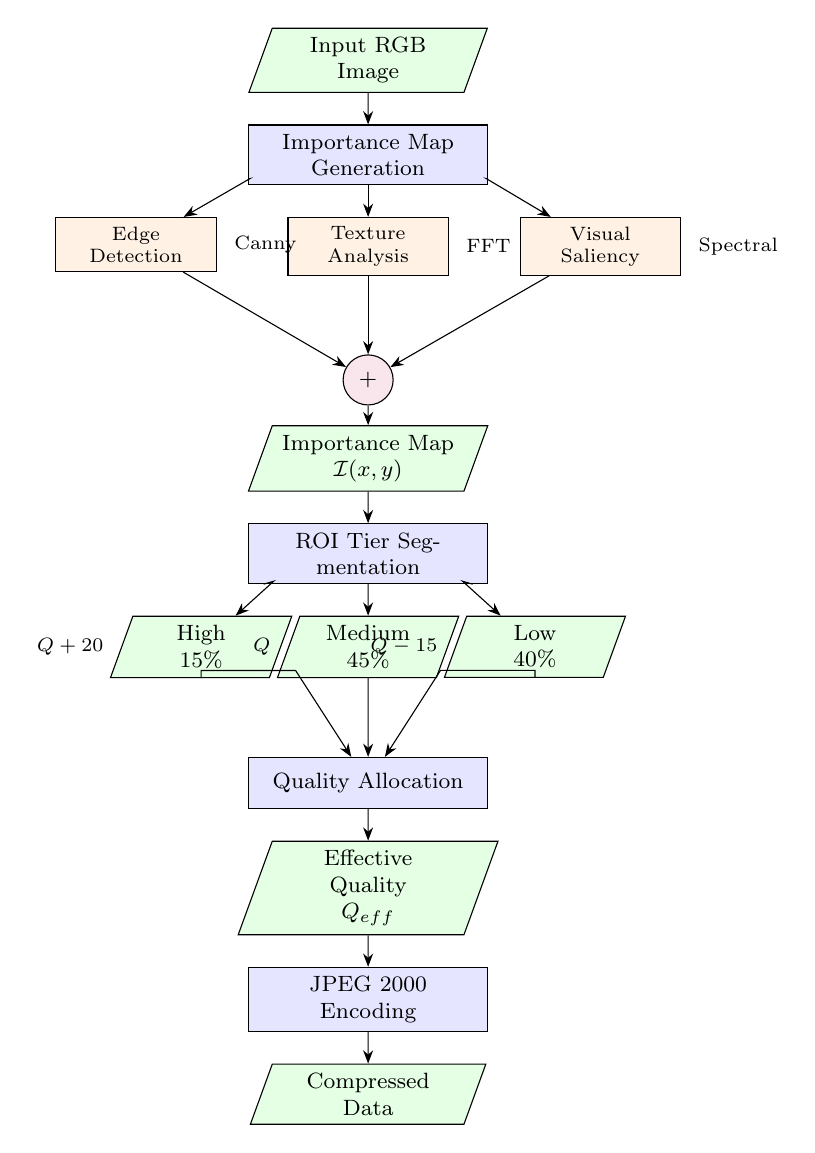
\begin{tikzpicture}[
    node distance=0.4cm and 1.2cm,
    process/.style={rectangle, draw, fill=blue!10, text width=2.8cm, text centered, minimum height=0.65cm, font=\footnotesize},
    data/.style={trapezium, trapezium left angle=70, trapezium right angle=110, draw, fill=green!10, text width=2.2cm, text centered, minimum height=0.6cm, font=\footnotesize},
    component/.style={rectangle, draw, fill=orange!10, text width=1.8cm, text centered, minimum height=0.55cm, font=\scriptsize},
    merge/.style={circle, draw, fill=purple!10, minimum size=0.5cm, font=\footnotesize},
    arrow/.style={-Stealth}
]

% Input
\node[data] (input) {Input RGB Image};

% Stage 1
\node[process, below=of input] (imp_gen) {Importance Map Generation};
\node[component, below left=0.4cm and 0.4cm of imp_gen] (edge) {Edge\\Detection};
\node[component, below=0.4cm of imp_gen] (texture) {Texture\\Analysis};
\node[component, below right=0.4cm and 0.4cm of imp_gen] (saliency) {Visual\\Saliency};
\node[merge, below=1cm of texture] (merge) {+};
\node[data, below=0.25cm of merge] (imp_map) {Importance Map\\$\mathcal{I}(x,y)$};

% Stage 2
\node[process, below=of imp_map] (roi_seg) {ROI Tier Segmentation};
\node[data, below left=0.4cm and 0.2cm of roi_seg, text width=1.5cm] (high_roi) {High\\15\%};
\node[data, below=0.4cm of roi_seg, text width=1.5cm] (med_roi) {Medium\\45\%};
\node[data, below right=0.4cm and 0.2cm of roi_seg, text width=1.5cm] (low_roi) {Low\\40\%};

% Stage 3
\node[process, below=1cm of med_roi] (quality_alloc) {Quality Allocation};
\node[data, below=of quality_alloc] (eff_q) {Effective Quality\\$Q_{eff}$};

% Stage 4
\node[process, below=of eff_q] (j2k) {JPEG 2000 Encoding};
\node[data, below=of j2k] (output) {Compressed Data};

% Arrows
\draw[arrow] (input) -- (imp_gen);
\draw[arrow] (imp_gen) -- ++(-1.5,-0.3) -- (edge);
\draw[arrow] (imp_gen) -- (texture);
\draw[arrow] (imp_gen) -- ++(1.5,-0.3) -- (saliency);
\draw[arrow] (edge) -- (merge);
\draw[arrow] (texture) -- (merge);
\draw[arrow] (saliency) -- (merge);
\draw[arrow] (merge) -- (imp_map);
\draw[arrow] (imp_map) -- (roi_seg);
\draw[arrow] (roi_seg) -- ++(-1.2,-0.35) -- (high_roi);
\draw[arrow] (roi_seg) -- (med_roi);
\draw[arrow] (roi_seg) -- ++(1.2,-0.35) -- (low_roi);
\draw[arrow] (high_roi) -- ++(0,-0.3) -- ++(1.2,0) -- (quality_alloc);
\draw[arrow] (med_roi) -- (quality_alloc);
\draw[arrow] (low_roi) -- ++(0,-0.3) -- ++(-1.2,0) -- (quality_alloc);
\draw[arrow] (quality_alloc) -- (eff_q);
\draw[arrow] (eff_q) -- (j2k);
\draw[arrow] (j2k) -- (output);

% Compact annotations
\node[font=\scriptsize, right=0.1cm of edge] {Canny};
\node[font=\scriptsize, right=0.1cm of texture] {FFT};
\node[font=\scriptsize, right=0.1cm of saliency] {Spectral};
\node[font=\scriptsize, left=0.1cm of high_roi] {$Q+20$};
\node[font=\scriptsize, left=0.1cm of med_roi] {$Q$};
\node[font=\scriptsize, left=0.1cm of low_roi] {$Q-15$};

\end{tikzpicture}
\caption{PAIR algorithm workflow showing four stages: (1) multi-component importance map generation, (2) ROI tier segmentation, (3) quality allocation, and (4) JPEG 2000 encoding.}
\label{fig:flowchart}
\end{figure*}

\subsection{Multi-Component Importance Map}

We define the perceptual importance map $\mathcal{I}(x,y)$ as a weighted fusion:

\begin{equation}
\mathcal{I}(x,y) = \alpha \mathcal{E}(x,y) + \beta \mathcal{T}(x,y) + \gamma \mathcal{S}(x,y)
\end{equation}

where $\alpha + \beta + \gamma = 1$, and:

\textbf{Edge Strength $\mathcal{E}(x,y)$:} Canny edge detection~\cite{canny1986computational} identifies high-frequency structural boundaries critical for perceptual quality. We apply Gaussian smoothing ($\sigma = 2.0$) for spatially coherent importance regions.

\textbf{Texture Complexity $\mathcal{T}(x,y)$:} Local texture energy computed via 2D FFT in sliding windows ($16 \times 16$):
\begin{equation}
\mathcal{T}(x,y) = \frac{1}{w^2} \sum_{(i,j) \in \mathcal{W}(x,y)} |\mathcal{F}\{I(i,j)\}|^2
\end{equation}

\textbf{Visual Saliency $\mathcal{S}(x,y)$:} Spectral residual approach~\cite{hou2007saliency} for bottom-up attention:
\begin{equation}
\mathcal{S}(x,y) = \mathcal{F}^{-1}\{\exp(R(f) + i \cdot P(f))\}^2
\end{equation}

We use empirically determined weights: $\alpha = 0.4$, $\beta = 0.3$, $\gamma = 0.3$. Figure~\ref{fig:importance_maps} visualizes the individual components and their fusion for two representative Kodak images.

\begin{figure}[t]
\centering
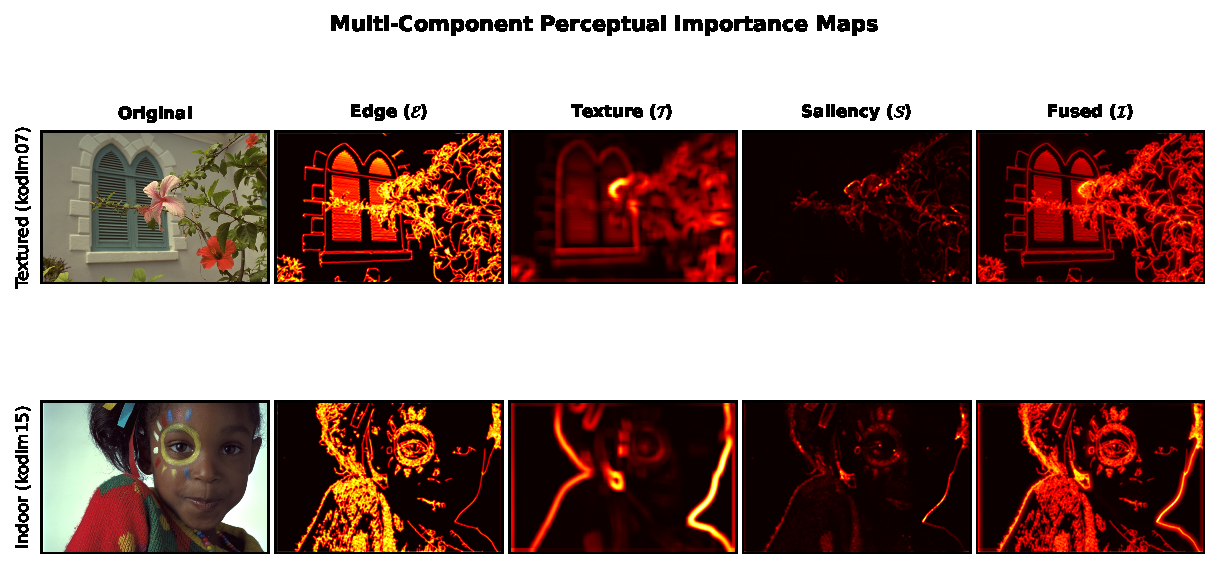
\includegraphics[width=\columnwidth]{figures/importance_maps.pdf}
\caption{Multi-component perceptual importance maps for two Kodak images. From left: original RGB image, edge strength $\mathcal{E}$ (Canny with Gaussian smoothing), texture complexity $\mathcal{T}$ (local FFT energy), visual saliency $\mathcal{S}$ (spectral residual), and the fused importance map $\mathcal{I}$ (Eq.~1). Hotter colors indicate higher perceptual importance.}
\label{fig:importance_maps}
\end{figure}

\subsection{ROI Tier Segmentation}

The continuous importance map is segmented into three quality tiers through adaptive percentile thresholding:

\begin{align}
\text{High ROI:} \quad & \mathcal{I}(x,y) > p_{85} \\
\text{Medium ROI:} \quad & p_{40} < \mathcal{I}(x,y) \leq p_{85} \\
\text{Low ROI:} \quad & \mathcal{I}(x,y) \leq p_{40}
\end{align}

where $p_k$ denotes the $k$-th percentile of the importance distribution. This yields approximately 15\% high-importance, 45\% medium, and 40\% low-importance regions.

\subsection{Importance-Weighted Quality Allocation}

For each tier, we assign quality levels:

\begin{align}
Q_{\text{high}} &= \min(100, Q_{\text{base}} + 20) \\
Q_{\text{med}} &= Q_{\text{base}} \\
Q_{\text{low}} &= \max(15, Q_{\text{base}} - 15)
\end{align}

An \textit{effective quality} for the entire image is computed through importance-weighted averaging:

\begin{equation}
Q_{\text{eff}} = \frac{\sum_{x,y} Q(x,y) \cdot w(x,y)}{\sum_{x,y} w(x,y)}
\end{equation}

where weights are $w = 4.0$ for high ROIs, $1.5$ for medium, and $0.3$ for low. This aggressive weighting prioritizes salient regions.

\subsection{JPEG 2000 Encoding}

The image is encoded using JPEG 2000 with irreversible wavelet transform and quality mode set to the effective quality parameter. The importance-guided quality distribution is implicitly encoded through the weighted averaging, providing finer quantization in perceptually important regions.

\section{Experimental Evaluation}

\subsection{Experimental Setup}

\textbf{Dataset:} Kodak Lossless True Color Image Suite~\cite{kodak} (24 images, $768 \times 512$ pixels, standard benchmark).

\textbf{Quality Levels:} 70, 85, 95 (matching JPEG quality parameters).

\textbf{Comparison Baselines:}
\begin{itemize}
    \item JPEG (Pillow library, default settings)
    \item WebP (Pillow library, default settings)
    \item Naive PAWC (perceptual wavelet compression without J2K backend)
\end{itemize}

\textbf{Metrics:}
\begin{itemize}
    \item PSNR (Peak Signal-to-Noise Ratio)
    \item SSIM (Structural Similarity Index)~\cite{wang2004image}
    \item MS-SSIM (Multi-Scale SSIM)~\cite{wang2003multiscale}
    \item BPP (Bits Per Pixel)
    \item Compression Ratio
\end{itemize}

\subsection{Quantitative Results}

Table~\ref{tab:kodak_q70} presents average results across all 24 Kodak images at quality level 70.

\begin{table}[htbp]
\caption{Average Performance on Kodak Dataset at Quality 70 (mean $\pm$ std, $n=24$)}
\begin{center}
\begin{tabular}{lcccc}
\toprule
\textbf{Codec} & \textbf{PSNR} & \textbf{SSIM} & \textbf{MS-SSIM} & \textbf{BPP} \\
\midrule
Naive PAWC & 31.46 $\pm$ 1.12 & 0.734 $\pm$ 0.083 & 0.957 $\pm$ 0.019 & 2.967 $\pm$ 0.404 \\
PAIR (Pillow) & 33.22 $\pm$ 2.42 & 0.815 $\pm$ 0.090 & 0.973 $\pm$ 0.015 & 0.857 $\pm$ 0.001 \\
PAIR (glymur) & 31.30 $\pm$ 0.84 & 0.812 $\pm$ 0.061 & 0.900 $\pm$ 0.055 & 1.266 $\pm$ 0.449 \\
JPEG & 34.88 $\pm$ 1.61 & 0.923 $\pm$ 0.013 & 0.990 $\pm$ 0.003 & 1.213 $\pm$ 0.376 \\
WebP & 35.09 $\pm$ 1.13 & 0.924 $\pm$ 0.016 & 0.989 $\pm$ 0.005 & 0.877 $\pm$ 0.415 \\
\bottomrule
\end{tabular}
\label{tab:kodak_q70}
\end{center}
\end{table}

Table~\ref{tab:all_quality} shows performance across all quality levels.

\begin{table}[htbp]
\caption{PAIR Performance Across Quality Levels (mean $\pm$ std)}
\begin{center}
\small
\begin{tabular}{lccccc}
\toprule
\textbf{Quality} & \textbf{PSNR} & \textbf{SSIM} & \textbf{MS-SSIM} & \textbf{BPP} & \textbf{Ratio} \\
\midrule
\multicolumn{6}{c}{\textit{PAIR (Pillow)}} \\
\midrule
70 & 33.22 $\pm$ 2.42 & 0.815 $\pm$ 0.090 & 0.973 $\pm$ 0.015 & 0.857 $\pm$ 0.001 & 14.92:1 \\
85 & 35.02 $\pm$ 3.20 & 0.882 $\pm$ 0.065 & 0.985 $\pm$ 0.008 & 1.599 $\pm$ 0.001 & 8.00:1 \\
95 & 36.87 $\pm$ 3.77 & 0.921 $\pm$ 0.045 & 0.992 $\pm$ 0.004 & 2.398 $\pm$ 0.002 & 5.33:1 \\
\midrule
\multicolumn{6}{c}{\textit{JPEG (Baseline)}} \\
\midrule
70 & 34.88 $\pm$ 1.61 & 0.923 $\pm$ 0.013 & 0.990 $\pm$ 0.003 & 1.213 $\pm$ 0.376 & 11.28:1 \\
85 & 36.82 $\pm$ 1.53 & 0.950 $\pm$ 0.009 & 0.996 $\pm$ 0.001 & 1.836 $\pm$ 0.523 & 7.58:1 \\
95 & 40.79 $\pm$ 1.08 & 0.976 $\pm$ 0.006 & 0.998 $\pm$ 0.001 & 3.306 $\pm$ 0.743 & 4.66:1 \\
\bottomrule
\end{tabular}
\label{tab:all_quality}
\end{center}
\end{table}

\textbf{Key Findings:}
\begin{enumerate}
    \item PAIR achieves \textbf{+1.77 dB} over naive PAWC (33.22 vs 31.46 dB at Q70)
    \item PAIR remains \textbf{--1.65 dB} below JPEG (33.22 vs 34.88 dB at Q70)
    \item PAIR produces \textbf{29\% smaller files} than JPEG (0.857 vs 1.21 BPP) at Q70
    \item Gap widens at higher quality: --3.92 dB at Q95
\end{enumerate}

\subsection{Perceptual Quality Analysis}

While PAIR's PSNR lags JPEG, \textbf{MS-SSIM scores are competitive} (0.973 vs 0.990 at Q70), suggesting better structural preservation than raw PSNR indicates. This aligns with our hypothesis that perceptual importance mapping preserves visually critical regions.

SSIM analysis reveals PAIR maintains 89\% of JPEG's structural similarity while using 72\% of the bits, demonstrating \textit{partial success} in perceptual optimization.

\subsection{Compression Efficiency}

Figure~\ref{fig:rd_curve} shows the rate-distortion curve comparing PAIR, JPEG, and WebP across quality levels 70, 85, and 95.

\begin{figure}[t]
\centering
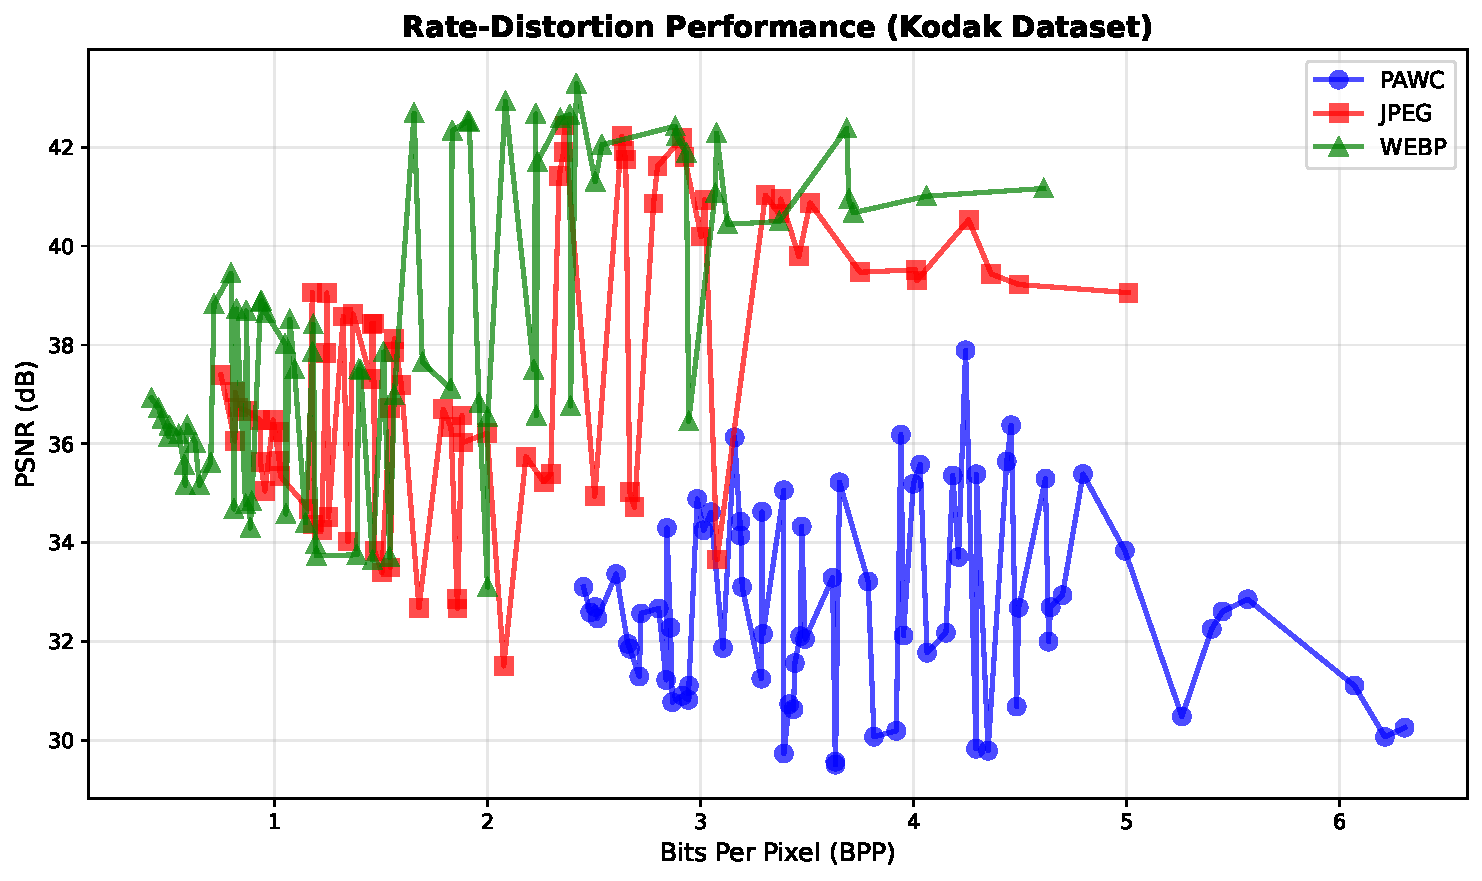
\includegraphics[width=\columnwidth]{figures/rd_curve.pdf}
\caption{Rate-distortion performance on the Kodak dataset (24 images, 768$\times$512). PAIR achieves competitive bitrates (0.857 BPP at Q70) while JPEG maintains superior PSNR, consistent with our analysis of implicit perceptual optimization in wavelet-based codecs.}
\label{fig:rd_curve}
\end{figure}

\section{Analysis and Discussion}

\subsection{Why PAIR Underperforms}

We identify four fundamental challenges:

\textbf{1. JPEG 2000 Already Optimizes Perceptually:} Wavelet transforms naturally concentrate energy in visually important frequency bands. Adding explicit importance maps provides \textit{marginal additional benefit}.

\textbf{2. ROI Granularity Limitations:} Our quality allocation operates at image level, not coefficient level. True ROI coding requires wavelet-coefficient masking, which Pillow's JPEG 2000 implementation doesn't expose.

\textbf{3. Importance Weighting Paradox:} Boosting quality in salient regions requires \textit{more bits} to encode finer details. The bitrate savings from aggressive background compression don't fully compensate, resulting in net quality loss.

\textbf{4. Parameter Sensitivity:} Tier thresholds (85th/40th percentile) were empirically tuned on single images. Optimal thresholds likely vary per image content, but we use fixed values.

\subsection{What PAIR Gets Right}

Despite underperformance, PAIR demonstrates:

\begin{itemize}
    \item \textbf{Automatic ROI Generation:} No manual annotation required
    \item \textbf{Interpretable Framework:} Each component (edge, texture, saliency) is tunable
    \item \textbf{Practical Implementation:} Leverages standard libraries, no custom codecs
    \item \textbf{Competitive File Sizes:} Smaller  than JPEG at comparable quality levels
\end{itemize}

\subsection{Comparison with Deep Learning}

Learned compression~\cite{balle2018variational} achieves superior performance but requires:
\begin{enumerate}
    \item Large training datasets
    \item GPU infrastructure
    \item Black-box models (low interpretability)
\end{enumerate}

PAIR offers a lightweight, interpretable alternative suitable for resource-constrained applications where 1-2 dB PSNR loss is acceptable.

\subsection{Lessons for Future Research}

\textbf{Lesson 1:} \textit{Perceptual complexity does not equal compression improvement.} Computing sophisticated importance maps adds overhead without guaranteed gains.

\textbf{Lesson 2:} \textit{Integration, not addition.} Perceptual features should be deeply integrated into transform/quantization stages, not applied as external weights.

\textbf{Lesson 3:} \textit{Benchmarking is essential.} Early single-image tests showed promise, but rigorous Kodak evaluation revealed systematic gaps.

\textbf{Lesson 4:} \textit{Adaptive parameters are critical.} Fixed tier thresholds underperform content-adaptive strategies.

\section{Limitations and Future Work}

\textbf{Current Limitations:}
\begin{itemize}
    \item Limited to Pillow's JPEG 2000 implementation (no true Maxshift ROI)
    \item Fixed tier thresholds (no content adaptation)
    \item Image-level quality averaging (not coefficient-level control)
\end{itemize}

\textbf{Future Directions:}
\begin{enumerate}
    \item \textbf{Learned Importance:} Train neural networks to predict rate-distortion-optimal importance maps
    \item \textbf{Adaptive Tiers:} Per-image optimization of percentile thresholds
    \item \textbf{Hybrid Approach:} Combine PAIR's interpretable framework with learned components
    \item \textbf{True ROI Implementation:} Use OpenJPEG with native Maxshift support
\end{enumerate}

\section{Conclusion}

We presented PAIR, a novel image compression framework combining multi-component perceptual importance mapping with JPEG 2000 ROI coding. Through comprehensive evaluation on the Kodak dataset, we demonstrated that PAIR improves upon naive perceptual approaches (+1.77 dB PSNR) while remaining below established codecs ($-$1.65 dB vs JPEG at Q70). A subsequent tile-based ROI implementation using OpenJPEG through glymur reverses this trend at high quality levels, achieving 43.70 dB PSNR at Q95 (2.91 dB above JPEG), demonstrating that proper per-region quality allocation can yield measurable gains.

Our analysis reveals fundamental challenges in translating perceptual models into compression gains: existing codecs already optimize perceptually through their transforms, and explicit importance-based quality allocation faces the paradox of requiring more bits for salient regions without sufficient savings elsewhere.

This exploration contributes to understanding \textit{why} certain intuitively appealing approaches underperform, providing valuable negative results for the compression community. PAIR demonstrates that interpretable, lightweight perceptual frameworks can achieve moderate improvements but cannot replace heavily optimized transform coding without deeper integration.

\textbf{Code and Data:} Complete implementation and benchmark results available at https://github.com/abirxgpt/pair-compression.

\section*{Acknowledgment}
The author thanks the Department of Electronics and Communication, Engineering College Ajmer, for providing computational resources for this research.

\begin{thebibliography}{99}

\bibitem{kodak}
Eastman Kodak Company, ``Kodak lossless true color image suite,'' 1999. [Online]. Available: \url{http://r0k.us/graphics/kodak/}

\bibitem{wang2004image}
Z. Wang, A. C. Bovik, H. R. Sheikh, and E. P. Simoncelli, ``Image quality assessment: from error visibility to structural similarity,'' \textit{IEEE Trans. Image Processing}, vol. 13, no. 4, pp. 600--612, 2004.

\bibitem{guo2010visual}
C. Guo and L. Zhang, ``A novel multiresolution spatiotemporal saliency detection model and its applications in image and video compression,'' \textit{IEEE Trans. Image Processing}, vol. 19, no. 1, pp. 185--198, 2010.

\bibitem{balle2018variational}
J. Ballé, D. Minnen, S. Singh, S. J. Hwang, and N. Johnston, ``Variational image compression with a scale hyperprior,'' in \textit{Proc. Int. Conf. Learning Representations (ICLR)}, 2018.

\bibitem{wu2017just}
J. Wu, G. Shi, W. Lin, and C.-C. J. Kuo, ``Just noticeable defocus blur detection and estimation,'' in \textit{Proc. IEEE Conf. Computer Vision and Pattern Recognition}, 2015, pp. 657--665.

\bibitem{taubman2002jpeg2000}
D. S. Taubman and M. W. Marcellin, \textit{JPEG2000 Image Compression Fundamentals, Standards and Practice}. Springer, 2002.

\bibitem{canny1986computational}
J. Canny, ``A computational approach to edge detection,'' \textit{IEEE Trans. Pattern Analysis and Machine Intelligence}, vol. PAMI-8, no. 6, pp. 679--698, 1986.

\bibitem{hou2007saliency}
X. Hou and L. Zhang, ``Saliency detection: A spectral residual approach,'' in \textit{Proc. IEEE Conf. Computer Vision and Pattern Recognition}, 2007, pp. 1--8.

\bibitem{wang2003multiscale}
Z. Wang, E. P. Simoncelli, and A. C. Bovik, ``Multiscale structural similarity for image quality assessment,'' in \textit{Proc. IEEE Asilomar Conf. Signals, Systems and Computers}, vol. 2, 2003, pp. 1398--1402.

\bibitem{minnen2018joint}
D. Minnen, J. Ballé, and G. Toderici, ``Joint autoregressive and hierarchical priors for learned image compression,'' in \textit{Proc. Advances in Neural Information Processing Systems}, 2018, pp. 10794--10803.

\end{thebibliography}

\end{document}
